\documentclass[11pt]{article}

% Preamble

\usepackage[margin=1in]{geometry}
\usepackage{amsfonts, amsmath, amssymb}
\usepackage{fancyhdr, float, graphicx}
\usepackage[utf8]{inputenc} % Required for inputting international characters
\usepackage[T1]{fontenc} % Output font encoding for international characters
\usepackage{fouriernc} % Use the New Century Schoolbook font
\usepackage[nottoc, notlot, notlof]{tocbibind}
\usepackage{listings}
\usepackage{xcolor}

\definecolor{codegreen}{rgb}{0,0.6,0}
\definecolor{codegray}{rgb}{0.5,0.5,0.5}
\definecolor{codepurple}{rgb}{0.58,0,0.82}
\definecolor{backcolour}{rgb}{0.95,0.95,0.92}

\lstdefinestyle{mystyle}{
    backgroundcolor=\color{backcolour},   
    commentstyle=\color{codegreen},
    keywordstyle=\color{magenta},
    numberstyle=\tiny\color{codegray},
    stringstyle=\color{codepurple},
    basicstyle=\ttfamily\footnotesize,
    breakatwhitespace=false,         
    breaklines=true,                 
    captionpos=b,                    
    keepspaces=true,                 
    numbers=left,                    
    numbersep=5pt,                  
    showspaces=false,                
    showstringspaces=false,
    showtabs=false,                  
    tabsize=2
}

\lstset{style=mystyle}

% Header and Footer
\pagestyle{fancy}
\fancyhead{}
\fancyfoot{}
\fancyhead[L]{\textit{\Large{FDS Assignment 4 - Bucket Sort and Radix Sort}}}
%\fancyhead[R]{\textit{something}}
\fancyfoot[C]{\thepage}
\renewcommand{\footrulewidth}{1pt}



% Other Doc Editing
% \parindent 0ex
%\renewcommand{\baselinestretch}{1.5}

\begin{document}

\begin{titlepage}
	\centering

	%---------------------------NAMES-------------------------------

	\huge\textsc{
		MIT World Peace University
	}\\

	\vspace{0.75\baselineskip} % space after Uni Name

	\LARGE{
		Fundamental Data Structures\\
		Second Year B. Tech, Semester 1
	}

	\vfill % space after Sub Name

	%--------------------------TITLE-------------------------------

	\rule{\textwidth}{1.6pt}\vspace*{-\baselineskip}\vspace*{2pt}
	\rule{\textwidth}{0.6pt}
	\vspace{0.75\baselineskip} % Whitespace above the title



	\huge{\textsc{
			Implementation of Bucket Sort
		}} \\



	\vspace{0.5\baselineskip} % Whitespace below the title
	\rule{\textwidth}{0.6pt}\vspace*{-\baselineskip}\vspace*{2.8pt}
	\rule{\textwidth}{1.6pt}

	\vspace{1\baselineskip} % Whitespace after the title block

	%--------------------------SUBTITLE --------------------------	

	\LARGE\textsc{
		Practical Report
	} % Subtitle or further description
	\vfill

	%--------------------------AUTHOR-------------------------------

	Prepared By
	\vspace{0.5\baselineskip} % Whitespace before the editors

	\Large{
		Krishnaraj Thadesar \\
		Cyber Security and Forensics\\
		Batch A2, PA 20
	}


	\vspace{0.5\baselineskip} % Whitespace below the editor list
	\today

\end{titlepage}


\tableofcontents
\thispagestyle{empty}
\clearpage


\setcounter{page}{1}

\section{Objectives}
\begin{enumerate}
	\item To understand use of an array of structures for maintaining records
	\item To implement, analyze and compare linear and binary search.
	\item To implement, analyze and compare selection, insertion sort and shell sort.
\end{enumerate}

\section{Problem Statements}
Write a C program to create a student database using an array of structures. Apply searching (Linear and Binary Search) and sorting techniques(Insertion Sort, Selection Sort, Shell sort).

\section{Theory}

\subsection{Bucket Sort}
Bucket Sort is a sorting algorithm that divides the unsorted array elements into several groups called buckets. Each bucket is then sorted by using any of the suitable sorting algorithms or recursively applying the same bucket algorithm.

Finally, the sorted buckets are combined to form a final sorted array.\\

\noindent
\textbf{Advantages of Bucket sort}
\begin{enumerate}
	\item It is simple and performs faster computation for numbers or strings
	\item Bucket sort can be used as an external sorting algorithm.
	\item Once the list is grouped in buckets then it can be processed independently.
\end{enumerate}
\textbf{Disadvantages of Bucket Sort}
\begin{enumerate}
	\item You can't apply it to all data types because you need a good bucketing scheme.
	\item Bucket sort's efficiency is sensitive to the distribution of the input values, so if you have tightly-clustered values, it's not worth it.
	\item In many cases where you could use bucket sort, you could also use another specialized sorting algorithm like radix sort, counting sort, or burstsort instead and get better performance.
	\item The performance of bucket sort depends on the number of buckets chosen, which might require some extra performance tuning compared to other algorithms.
\end{enumerate}
\subsection{Example}
Here is an Example of how Bucket Sort Works.
\begin{figure}[H]
	\centering
	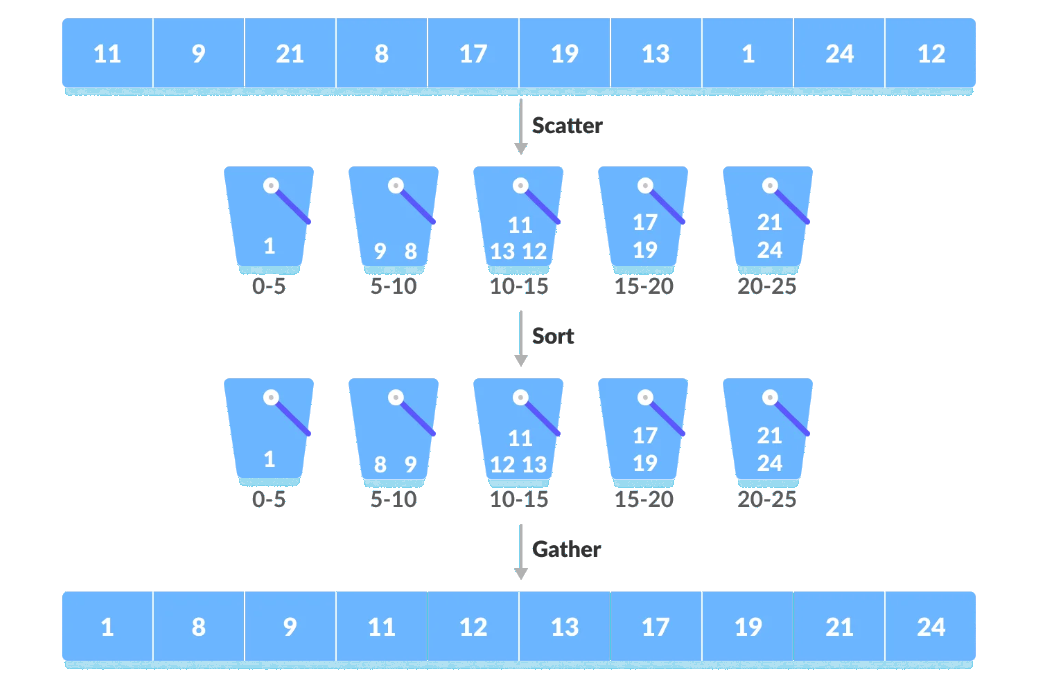
\includegraphics[scale=0.5]{bucket_workinge.png}
	\caption{An Example of the Working of Bucket Sort}
\end{figure}
\section{Platform}
\textbf{Operating System}: Arch Linux x86-64 \\
\textbf{IDEs or Text Editors Used}: Visual Studio Code\\
\textbf{Compilers} : gcc on linux for C\\

\section{Input}

\begin{itemize}
	\item Array of Integer Elements
	\item Array of Floating Point Elements
\end{itemize}

\section{Output}
\begin{itemize}
	\item Sorted Elements
\end{itemize}

\section{Test Conditions}
\begin{enumerate}
	\item Input at least 10 records.
	\item Test bucket sorting methods for at least 10 records.
\end{enumerate}

\section{Code}
\subsection{Pseudo Code}

\subsubsection{Pseudo Code for Implementation of Bucket Sort}
\begin{lstlisting}[language=C]
void bucket_sort_integers(int arr[], int size)
{
	max = find_max(arr, size) + 1;
	int bucket[max];
	for (int i = 0; i < max; i++)
		bucket[i] = 0;
	for (int i = 0; i < size; i++)
		bucket[arr[i]]++ 
	for (int i = 0, j = 0; i < max; i++)
		for (; bucket[i] > 0; bucket[i]--)
		{
			arr[j] = i
			j++
		}
}
\end{lstlisting}
\subsection{C Implementation of Problem Statement}

\lstinputlisting[language=c++, caption=Main.Cpp]{../Programs/[Krishnaraj]_[FDS]_Assignment_4.c}

\subsection{C Output}
\lstinputlisting[caption=Output]{../Programs/[Krishnaraj]_[FDS]_Assignment_4_output.txt}

\section{Time Complexity}
\textbf{Worst Case Complexity: O(n2)}\\
When there are elements of close range in the array, they are likely to be placed in the same bucket. This may result in some buckets having more number of elements than others.
It makes the complexity depend on the sorting algorithm used to sort the elements of the bucket.
The complexity becomes even worse when the elements are in reverse order. If insertion sort is used to sort elements of the bucket, then the time complexity becomes O(n2).\\

\noindent
\textbf{Best Case Complexity: O(n+k)}\\
It occurs when the elements are uniformly distributed in the buckets with a nearly equal number of elements in each bucket.
The complexity becomes even better if the elements inside the buckets are already sorted.
If insertion sort is used to sort elements of a bucket then the overall complexity in the best case will be linear ie. O(n+k). O(n) is the complexity for making the buckets and O(k) is the complexity for sorting the elements of the bucket using algorithms having linear time complexity at the best case.\\

\noindent
\textbf{Average Case Complexity: O(n)}\\
It occurs when the elements are distributed randomly in the array. Even if the elements are not distributed uniformly, bucket sort runs in linear time. It holds true until the sum of the squares of the bucket sizes is linear in the total number of elements.

\section{Conclusion}
Thus, implemented bucket sort and Radix Sort Algorithm

\section{FAQs}
\begin{enumerate}
	\item What are the applications of bucket sort?
	      Bucket sort is used when:
	      \begin{itemize}
		      \item Input is uniformly distributed over a range.
		      \item There are floating point values
	      \end{itemize}
	\item Compare bucket sorting with other sorting methods?
	      \begin{enumerate}
		      \item Bucket sort is different from other algorithms that we have learnt, in that it is not a comparison based algorithm like Bubble or selection sort.
		      \item The advantage of bucket sort is that once the elements are distributed into buckets, each bucket can be processed independently of the others. This means that you often need to sort much smaller arrays as a follow-up step than the original array.
		      \item Another advantage of bucket sort is that you can use it as an external sorting algorithm. If you need to sort a list that is so huge you can't fit it into memory, you can stream the list through RAM, distribute the items into buckets stored in external files, then sort each file in RAM independently.
		      \item You can't apply it to all data types because you need a good bucketing scheme.
		      \item Worst Case time Complexity is same as that of Bubble, Selection, Insertion and Quick sort.
		      \item Average Case Time Complexity is better than above mentioned algorithms.
		      \item Best Case time complexity is $\Omega(n + k)$ which is worse than above mentioned algorithms, but better than selection sort.
	      \end{enumerate}
\end{enumerate}
\end{document}